\documentclass[11pt,a4paper]{article}
\usepackage[T1]{fontenc}
\usepackage{lmodern,amsmath,amssymb,amsthm,booktabs,microtype,graphicx}
\usepackage[margin=24mm]{geometry}
\usepackage[colorlinks=true,urlcolor=blue,linkcolor=blue]{hyperref}
\newcommand{\Js}{\mathcal J_s}
\newcommand{\E}{\mathbb E}
\newcommand{\tr}{\operatorname{tr}}
\newcommand{\av}[1]{\langle #1\rangle}
\newcommand{\K}{\mathsf K}
\DeclareMathOperator{\sech}{sech}
\title{The linear cubic residual has a full $q$ kernel\\A covariance bridge to existing embedded ensembles}
\author{Alan Day \and Chengheng\thanks{AI research assistant (OpenAI).}}
\date{Local research note --- 6 November 2026}
\begin{document}\maketitle
\begin{abstract}
The first Gaussian-chaos residual of the cubic derivative singlet
is a deterministic linear filter of the same couplings as its
Hamiltonian. We prove that its joint fixed-degree moments with the
Hamiltonian nevertheless tend to those of two orthogonal
$q$-Gaussian variables. The proof approximates the three covariance
blocks in rank-weight total variation by finite combinations of
existing embedded ensembles of body orders $p,p-1,p-2$.
A uniform diagram bound controls the replacement before taking
the double-scaled limit. The known Mehler kernel then gives the
complete two-point function and the small-coupling limit
$\sech^2(2\Js t)$.
\end{abstract}

\section{Result and place in the singlet construction}
Use standard CAR, the complex Gaussian number-preserving
$p$-body Hamiltonian $H=H_s$, all overlapping index sets included,
and infinite temperature at zero chemical potential. Time is
conjugate to $H_s$, with $\hbar=1$. Define
\[
 T_3=\tfrac12\left(\sum_i c_i^\dagger[H,[H,[H,c_i]]]
                 +\mathrm{h.c.}\right),\qquad
 F=\mathcal W_1T_3-\bar t(Q_f)H.
\]
$\mathcal W_1$ is ordinary Gaussian coupling chaos; $\bar t$ is
the sector-wise ensemble projection coefficient. The preceding
notes give its exact rank coefficients, its positive norm and
second dynamic moment \cite{local}.
Take DS first, $p^2/N=\lambda>0$, and write
\[
 q=e^{-4\lambda},\qquad \sigma^2=\Js^2/\lambda,
 \qquad V=\av{F^2}_{\rm DS}=64\Js^6q^2.
\]
For every fixed word $w$ in $h=H/\sigma$ and $y=F/\sqrt V$,
\begin{equation}
 \boxed{\av{w(h,y)}_{\rm DS}
 =\sum_{\substack{\pi\text{ pairs the slots of }w\\
                   \text{each pair has equal letters}}}
 q^{\operatorname{cr}(\pi)}.}                 \label{joint}
\end{equation}
The sum is zero for odd length. This is a moment statement, not
finite-size statistical independence. In particular the full
two-point kernel is the existing probe kernel with $r=q$, and
\begin{equation}
 \boxed{\lim_{\lambda\to0^+}
 \frac{\av{F(t)F(0)}_{\rm DS}}{V}
 =\sech^2(2\Js t).}                           \label{limit}
\end{equation}

\newpage
\section{Rank weights and three covariance blocks}
Work first at $m=N/2$, with normalized sector trace. For
$r\leq\min(m,N-m)$, the unit-variance embedded ensemble has
covariance tensor
\begin{equation}
 \K_r=\sum_{a=0}^r\omega_a^{(r)}\mathsf Q_a,\qquad
 \omega_a^{(r)}=
 \frac{d_a\binom{m-a}{m-r}\binom{N-r-a}{m-r}}
 {\binom Nm\binom mr\binom{N-m+r}{r}},          \label{weights}
\end{equation}
where $d_a=\binom Na^2-\binom N{a-1}^2$.
$\mathsf Q_a$ is the covariance of a unit-variance Hermitian
Gaussian operator of pure $U(N)$ rank $a$; in particular
$\E A_a^2=\mathbf1$. These are the standard covariance components
of the embedded ensemble \cite{kota}.

Let $C_m=\E\tr_m H^2$, $H=\sum_a H_a$,
$\E\tr_m H_a^2=C_m\omega_a^{(p)}$ and
$F=\sum_a(t_a-\bar t)H_a$. Set
\[
 c_a=t_a/C_m,\quad
 \delta_a=c_a-\sum_b\omega_b^{(p)}c_b,\quad
 W_N=\sum_a\omega_a^{(p)}\delta_a^2.
\]
The exactly normalized sector variables are
$h_N=H/\sqrt{C_m}$ and $y_N=F/\sqrt{C_m^3W_N}$.
With $u_a=\delta_a/\sqrt{W_N}$, their covariances are
\begin{equation}
 \K_{hh}=\sum_a\omega_a\mathsf Q_a,\quad
 \K_{hy}=\sum_a\omega_a u_a\mathsf Q_a,\quad
 \K_{yy}=\sum_a\omega_a u_a^2\mathsf Q_a.       \label{blocks}
\end{equation}
Although $\sum\omega_a u_a=0$, $\K_{hy}$ is generally not zero.
Consequently scalar energy projection alone does not permit
using an independent-probe formula.

The preceding rank calculation proves, with all polynomial moments,
\begin{equation}
 s=p-a\Longrightarrow\operatorname{Poisson}(\lambda),\qquad
 u_{p-s}\longrightarrow\frac{s-\lambda}{\sqrt\lambda}.
                                                               \label{poisson}
\end{equation}
It also supplies uniform bounds
$\omega_{p-s}\leq K_\lambda(32\lambda)^s/s!$ and
$|u_{p-s}|\leq K_\lambda(1+s)$ for sufficiently large $N$.

An exact finite-size ratio connects these polynomial weights
to familiar ensembles. For fixed integer $j\geq0$, define
\begin{equation}
 R_j(s)=\frac{\omega_{p-s}^{(p-j)}}{\omega_{p-s}^{(p)}}
 =\frac{s^{\underline j}(N-2p+s+1)^{\overline j}
                 (N-m+p-j+1)^{\overline j}}
 {(m-p+1)^{\overline j}(p^{\underline j})^2}.    \label{ratio}
\end{equation}
The numerator is zero for $s<j$; bars denote rising and
underlines falling factorials. For fixed $s,j$,
$R_j(s)\to s^{\underline j}/\lambda^j$, and
$R_j(s)\leq K_{\lambda,j}(1+s)^j$ uniformly.

\newpage
\section{The finite covariance bridge}
For signed rank covariances define
$\|\sum_a z_a\mathsf Q_a\|_{\rm rv}=\sum_a|z_a|$.
This measures the total variation of their scalar rank weights.
Equations \eqref{poisson}--\eqref{ratio} and the factorial tail give
\begin{align}
 \K_{hh}&=\K_p,\nonumber\\
 \K_{hy}&=\sqrt\lambda(\K_{p-1}-\K_p)+o_{\rm rv}(1),
                                                               \label{hy}\\
 \K_{yy}&=\lambda\K_{p-2}+(1-2\lambda)\K_{p-1}
                         +\lambda\K_p+o_{\rm rv}(1).            \label{yy}
\end{align}
Indeed the associated ratios to $\omega_{p-s}^{(p)}$ tend to
$(s-\lambda)/\sqrt\lambda$ and $(s-\lambda)^2/\lambda$,
respectively. The second equality uses
$s^2=s^{\underline2}+s$. Dominated convergence proves the
total-variation statements, including the normalization $W_N$.
For $\lambda>1/2$ one coefficient in \eqref{yy} is negative.
These are signed covariance substitutions in individual Wick
diagrams, not a proposed positive Gaussian ensemble.

\paragraph{A bound for an entire diagram.}
Consider a fixed pairing $\pi$ with $n$ chords. For positive
unit-variance covariance on each chord, represent distinct
chords by independent Hermitian Gaussian matrices $A_1,\ldots,A_n$.
The diagram is the expectation of a normalized trace word in
which each $A_j$ occurs twice. Tracial H\"older and the Gaussian
matrix bound $\E\tr A_j^{2n}\leq(2n-1)!!$ give
\begin{equation}
 |D_\pi(\mathsf Q_{a_1},\ldots,\mathsf Q_{a_n})|
 \leq (2n-1)!!=:B_n.                          \label{bound}
\end{equation}
The Gaussian bound was proved by integration by parts in the
preceding dynamics note; it uses only $\E A_j^2=\mathbf1$.
Expanding signed rank weights extends \eqref{bound} to
$B_n\prod_j\|\K_j\|_{\rm rv}$.

Let $\epsilon_N$ be the larger error in \eqref{hy}, \eqref{yy}.
The actual covariance norms are at most one; the substituted
ones are at most
\[
 B=\max\{1,2\sqrt\lambda,2\lambda+|1-2\lambda|\}.
\]
A telescoping replacement of the $n$ edges therefore changes
one diagram by at most
\begin{equation}
 n B_n B^{n-1}\epsilon_N\longrightarrow0.       \label{error}
\end{equation}
This bound is uniform in the ranks being summed. Thus the
covariance bridge controls arbitrary fixed words, rather than
only one crossing or a finite list of frequency moments.

\paragraph{The imported diagram law.}
For independent unit-variance embedded ensembles with body orders
$r_j=p-j_j$, where every $j_j$ is fixed, the existing DS chord
rule gives $D_\pi\to q^{\operatorname{cr}(\pi)}$.
In the general-body rule the pair crossing weight is
$\exp[-r_ir_j/(N\rho(1-\rho))]$, $\rho=m/N$; here
$\rho=1/2$ and $r_i/p\to1$ \cite{tall,bnr}.
The number of chords is held fixed. The covariance bridge
reduces our correlated operator to precisely these established
independent-ensemble diagrams.

\newpage
\section{All-order cancellation and a rank-filter interpretation}
After \eqref{hy}--\eqref{yy}, each diagram is a finite sum of
body-shift choices. Every choice has the same limiting
factor $q^{\operatorname{cr}(\pi)}$. The coefficient sum on one
edge is
\begin{equation}
 hh:1,\qquad hy:\sqrt\lambda(1-1)=0,\qquad
 yy:\lambda+(1-2\lambda)+\lambda=1.             \label{sums}
\end{equation}
Consequently any pairing containing a mixed $h$--$y$ edge
vanishes in the limit. The other pairings each give the usual
$q^{\operatorname{cr}}$. Together with \eqref{error}, this proves
\eqref{joint}. It does not assume that Gaussian chaos is preserved
under time evolution.

The full infinite-temperature trace follows by restricting first
to $|m-N/2|\leq N^{2/3}$. On that window the covariance limits,
sector normalizations and diagram bounds are uniform. Outside it,
the binomial charge probability decays faster than the polynomial
bounds on $t_a$ and all fixed Gaussian moments. Thus the
full-trace $h,y$ in \eqref{joint} have the stated limit.

For $P_{uv}(q,r)$, the standard unit-variance probe moment,
the immediate two-insertion consequence is
\begin{equation}
 \av{FH^uFH^v}_{\rm DS}=V\sigma^{u+v}P_{uv}(q,q).
                                                               \label{twoarc}
\end{equation}
At total Hamiltonian degree four,
\begin{align}
 P_{40}&=2+q,&P_{31}&=q(2+q),&P_{22}&=1+q^2(1+q),\\
 \mu_{4,F}&=\frac{2\Js^4}{\lambda^2}(1-q)^2(3q+5)
                 \longrightarrow256\Js^4.                    \label{fourth}
\end{align}
Also $\av{y^4}=2+q$ and $\av{hyhy}=q$.

\paragraph{A useful extension of the construction.}
For fixed polynomials $P_i$, consider the rank filters
$Y_{i,N}=\sum_a P_i(p-a)H_a/\sqrt{C_m}$.
Each edge covariance contains $P_i(s)P_j(s)$. Expand this
finite polynomial in falling factorials and use \eqref{ratio}
with the required finite set of shifts. The same diagram argument
gives a $q$-Gaussian family with covariance
\[
 G_{ij}=\E_{s\sim\operatorname{Poisson}(\lambda)}P_i(s)P_j(s).
\]
In particular orthonormal Charlier polynomials produce orthogonal
variables in this limiting moment algebra. $h$ corresponds to
$P_0=1$, and $y$ to $P_1=(s-\lambda)/\sqrt\lambda$.
This extension concerns explicit rank filters of $H$. Identifying
which of them arise in the local derivative-singlet tower is a
separate physical construction, not an automatic particle count.

\newpage
\section{The existing kernel now applies to $F$}
Set $(z;q)_\infty=\prod_{j\geq0}(1-zq^j)$, and define
\begin{align}
 \rho_q(\theta)&=\frac{(q,e^{2i\theta},e^{-2i\theta};q)_\infty}{2\pi},
 &E(\theta)&=\frac{2\sigma\cos\theta}{\sqrt{1-q}},\\
 \mathcal K_r(\theta,\phi)&=
 \frac{(r^2;q)_\infty}
 {\prod_{\varepsilon,\varepsilon'=\pm1}
 (r e^{i(\varepsilon\theta+\varepsilon'\phi)};q)_\infty},
 &r&=q.
\end{align}
The known positive Mehler measure \cite{tall,bnr} gives
\begin{equation}
 C_F(t)=\int_0^\pi\!\!\int_0^\pi
 \rho_q(\theta)\rho_q(\phi)\mathcal K_q(\theta,\phi)
 e^{it(E(\theta)-E(\phi))}\,d\theta\,d\phi.       \label{kernel}
\end{equation}
The normalization is $C_F(0)=1$. This formula is imported after
proving the operator-to-probe correspondence, not asserted from
the second frequency moment.

At finite size the normalized two-energy measure is
$V_N^{-1}\E\tr[F\,d\Pi_H(E)F\,d\Pi_H(E')]$.
It is positive. Equation \eqref{twoarc} determines all its
limiting mixed moments. The second energy moments give tightness;
higher even moments give uniform integrability for each monomial.
The candidate measure in \eqref{kernel} has compact support and
is moment determinate, so the measures converge weakly to it.
The bounded continuous characteristic function proves
\eqref{kernel} at every fixed real time.

For $0<q<1$ this measure is absolutely continuous. Its frequency
pushforward has support
$|\omega|\leq4\sigma/\sqrt{1-q}$ and no atom at zero.
Portmanteau on the closed diagonal shows that the normalized
finite-size exactly static weight tends to zero as well.
This strengthens the previous result, which only established
positive surviving dynamic weight.

For stable evaluation the equivalent Jacobi representation is
\begin{equation}
 C_F(t)=\sum_{n\geq0}q^n
 |\langle n|e^{-itT_q}|0\rangle|^2,\qquad
 (T_q)_{n-1,n}=\sigma\sqrt{\frac{1-q^n}{1-q}}.   \label{jacobi}
\end{equation}
The known small-coupling probe limit with $r=q^d$, or the
fixed-descendant contraction in our preceding note, applies with
$d=1$ \cite{small,local}. Its Liouvillian ladder entries are
$2\Js\sqrt{(n+1)(n+2)}$, giving \eqref{limit}.
In the convention $C(t)=\int S(\omega)e^{it\omega}d\omega/(2\pi)$,
\begin{equation}
 S_1(\omega)=\frac{\pi\omega}{4\Js^2\sinh(\pi\omega/(4\Js))},
 \qquad S_1(0)=\frac1{\Js}.                    \label{fourier}
\end{equation}
This is a frequency spectrum in string-time units, not a bulk
mass spectrum. The equal-time ratio of the $F$ and $R$ strengths
remains $2\lambda+o(\lambda)$, as obtained previously.

\newpage
\section{Computed evidence and next physical calculation}
\begin{center}
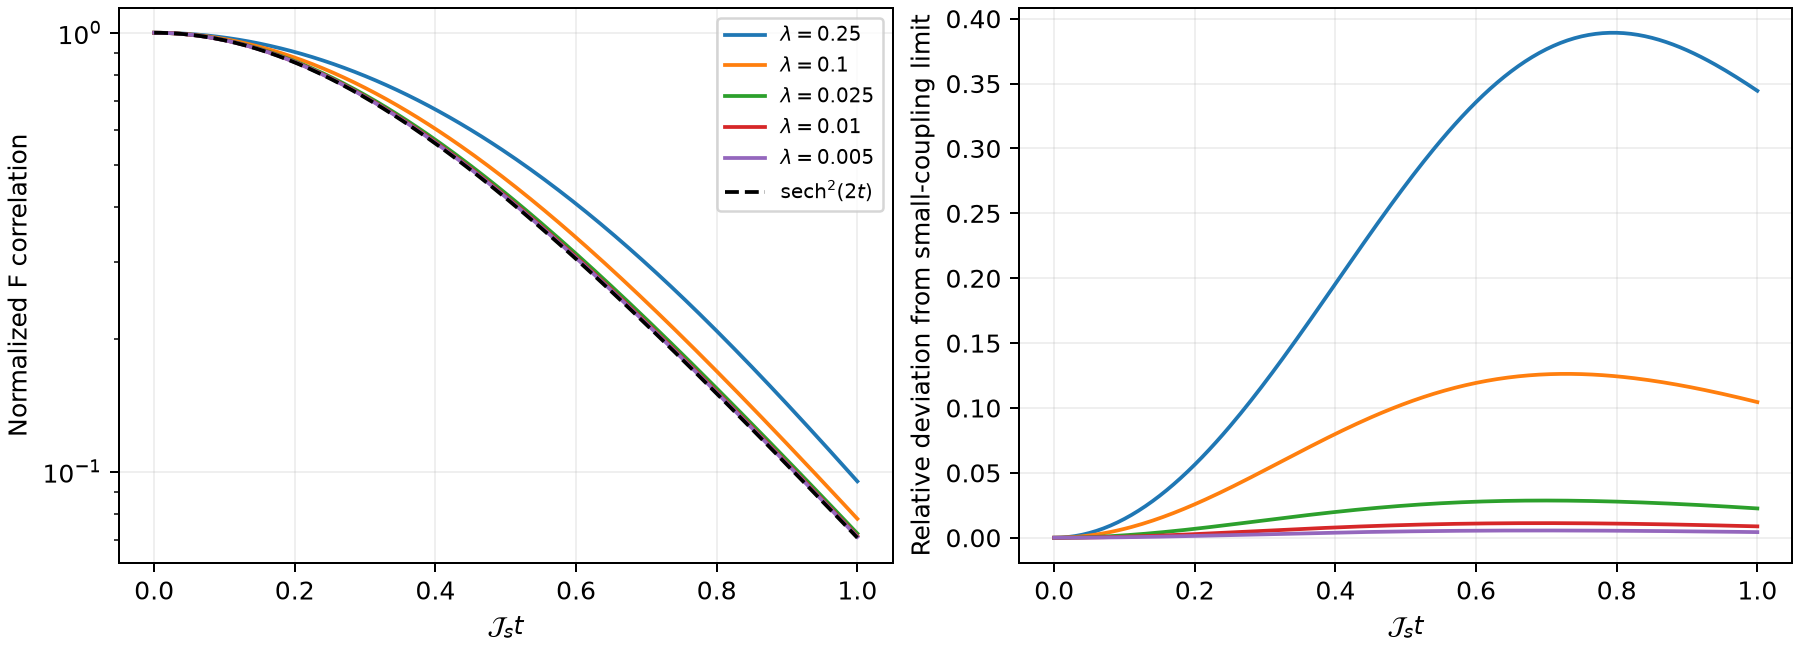
\includegraphics[width=\linewidth]{../../results/susskind-linear-kernel/correlation.png}
\end{center}
The full-rank covariance replacement errors are evaluated without
a deficit cutoff. At $p=256$:
\begin{center}
\begin{tabular}{rrr}
\toprule
$\lambda$ & $\|\Delta\K_{hy}\|_{\rm rv}$ & $\|\Delta\K_{yy}\|_{\rm rv}$\\
\midrule
0.10 & $8.4170\,10^{-5}$ & $9.3549\,10^{-4}$\\
0.25 & $6.5917\,10^{-4}$ & $1.2584\,10^{-3}$\\
0.50 & $2.4968\,10^{-3}$ & $3.8296\,10^{-3}$\\
1.00 & $8.5851\,10^{-3}$ & $1.7252\,10^{-2}$\\
\bottomrule
\end{tabular}
\end{center}
There are 2,286 exact rational ratio checks of \eqref{ratio} and
20 full-rank cases at 80/120 working digits. Agreement is checked
on 65-digit saved values; it is not a rounding certificate.

The finite-CAR calculation evaluates every one of the 15 Gaussian
pairings in each six-slot word $FH^uFH^{4-u}$, in three systems.
It retains the mixed-pair contributions separately and rechecks
the preceding degree-two results. For $(N,p,m)=(5,2,3)$ and
coupling variance one, it gives the exact values
$\av{F^2}=180$ and $\av{FL^4F}=314280$.
These finite-size numbers are not equated to their DS limits.

Five Jacobi computations use $\lambda=.25,.1,.025,.01,.005$,
cutoffs $33,52,138,302,574$, and refinements by 16 levels.
The analytic Taylor-tail bound is below $10^{-13}$.
Independent 128/192-node Mehler quadrature verifies the function
and its first two nontrivial moments for $\lambda=.25,.1$.
Four Fourier integrals are checked at 50/80 digits.
At $\lambda=.005$ the largest relative difference from
$\sech^2(2t)$ on $0\leq t\leq1$ is still about $0.560\%$.
All finite-coupling differences are retained. Float refinement
and quadrature comparisons are empirical precision checks.

The next calculation is the real-time cross spectrum of $F$
with the cubic third-chaos terms $R,S,Z$. The theorem here concerns
the $(H,F)$ moment algebra; it does not yet combine the raw
$M_3=R+aS+bZ+\bar t(Q_f)H+F+\tfrac32LA$ spectrum. After that,
the mixed $X,R,F$ interactions and the spatial translation
dictionary remain the route to the Susskind bulk construction.
This stage was saved locally without a Git commit or push.

\newpage
\section*{Sources and proof dependencies}
The proof imports the standard independent-ensemble chord law,
not finite-size independence of $F$. The additional step is the
rank-weight covariance approximation and its diagram bound.
The asymptotic rank distribution and the exact filter $t_a$
come from our preceding local notes. The Mehler formula and
small-coupling probe kernel are existing results.

Nine further full-rank computations evaluate the entire quartic
polynomial $\av{(h_N+z y_N)^4}$, including its odd mixed
coefficients, at 80/120 digits. They approach
$(2+q)(1+z^2)^2$; all finite-size deviations are stored.
This directly tests the joint-law prediction in addition to the
two-insertion curvature.

The first curve-generation run stopped during plotting because
of a malformed math-text axis label. The label was corrected;
the numerical tolerances were unchanged. The failure record,
successful data, code hashes, compiler logs and reviewed page
hashes are retained with the local evidence.

\begin{thebibliography}{9}
\bibitem{local} A. Day and Chengheng, local notes:
\emph{The missing linear component of the cubic singlet};
\emph{Dynamics of the linear cubic residual};
\emph{A positive chord generator from the tracial seed}.
See \texttt{manuscript/susskind-cubic-linear},
\texttt{susskind-cubic-dynamics}, and \texttt{susskind-antisymmetric}.
\bibitem{kota} V. K. B. Kota,
\emph{Bivariate moments of the two-point correlation function for
embedded Gaussian unitary ensemble with $k$-body interactions},
\href{https://arxiv.org/html/2208.11312}{arXiv:2208.11312v2},
Sec. IV, Eqs. (28)--(31).
\bibitem{tall} J. Tall and S. Tomsovic,
\emph{Double-scaled bosonic and fermionic embedded ensembles,
complex SYK, and the dual Hilbert space},
\href{https://arxiv.org/html/2604.14522v2}{arXiv:2604.14522v2},
Sec. 2.1, Eqs. (2.17)--(2.21); Sec. 4.1,
Eqs. (4.3), (4.15)--(4.18).
\bibitem{bnr} M. Berkooz, P. Narovlansky and H. Raj,
\emph{Complex Sachdev--Ye--Kitaev model in the double scaling limit},
\href{https://arxiv.org/html/2006.13983v2}{arXiv:2006.13983v2},
Secs. 3.2--3.3 (generic index-set lengths), 7 and 8.1.
\bibitem{small} B. Mukhametzhanov,
\emph{Large p SYK from chord diagrams},
\href{https://arxiv.org/abs/2303.03474v3}{arXiv:2303.03474v3},
Sec. 4; conventions here are $-\log q=4\lambda$,
$J_{\rm source}=2\Js$ at infinite temperature.
\end{thebibliography}
\end{document}
